\subsection{Results}

\begin{frame}{Evaluation Methodology}
    \begin{itemize}
        \item \textbf{Dataset}: Validation set from the before-mentioned dataset
        \item \textbf{Degradation}: Motion blur with varying kernel sizes
        \item \textbf{Methods Compared}:
              \begin{itemize}
                  \item DPS (Diffusion Posterior Sampling)
                  \item RED-Diff (Regularization by Denoising)
              \end{itemize}
        \item \textbf{Evaluation Metrics}:
              \begin{itemize}
                  \item PSNR (Peak Signal-to-Noise Ratio) in dB
                  \item SSIM (Structural Similarity Index)
              \end{itemize}
    \end{itemize}
\end{frame}

\begin{frame}{Setup and Configuration}
    \begin{itemize}
        \item \textbf{Motion Blur Configuration}:
              \begin{itemize}
                  \item Kernel sizes tested: [5, 7, 9, 11, 13, 15] pixels
                  \item Motion angle: 45°
                  \item Kernel type: Linear motion blur
              \end{itemize}
        \item \textbf{Evaluation Protocol}:
              \begin{itemize}
                  \item 5 images per kernel size for statistical reliability
                  \item Batch size: 1 (individual image processing)
              \end{itemize}
    \end{itemize}
\end{frame}

\begin{frame}{Metric Computation Process}
    \begin{itemize}
        \item \textbf{For each test image}:
              \begin{enumerate}
                  \item Load ground truth image $x_{gt}$
                  \item Apply motion blur: $y = K(x_{gt})$
                  \item Reconstruct using DPS: $x_{dps} = \text{DPS}(y, K)$
                  \item Reconstruct using RED-Diff: $x_{red} = \text{RED-Diff}(y, K)$
                  \item Compute metrics: $\text{PSNR}(x_{gt}, x_{rec})$, and $\text{SSIM}(x_{gt}, x_{rec})$
              \end{enumerate}
    \end{itemize}
\end{frame}

\begin{frame}{PSNR}
    Figure \ref{fig:psnr_results} shows the PSNR values for both methods across different kernel sizes.
    \begin{figure}
        \centering
        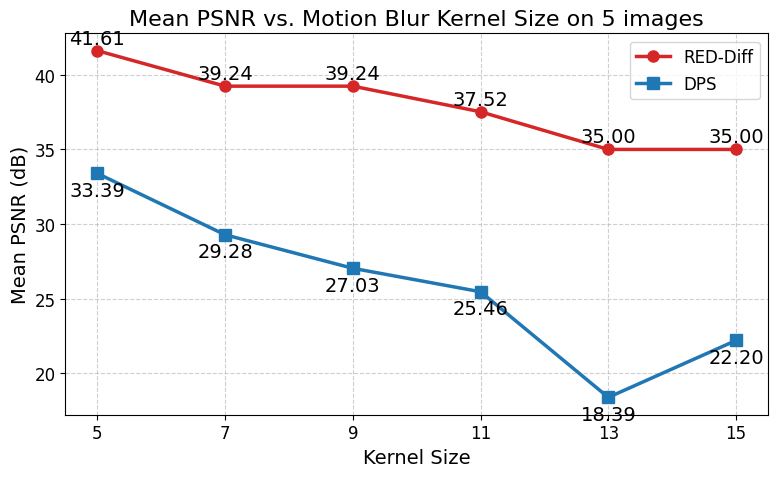
\includegraphics[width=0.5\textwidth]{media/mean_psnr_over_kernels.png}
        \caption{PSNR values for DPS and RED-Diff across different kernel sizes.}
        \label{fig:psnr_results}
    \end{figure}
\end{frame}

\begin{frame}{SSIM}
    Figure \ref{fig:ssim_results} illustrates the SSIM values for both methods across different kernel sizes.
    \begin{figure}
        \centering
        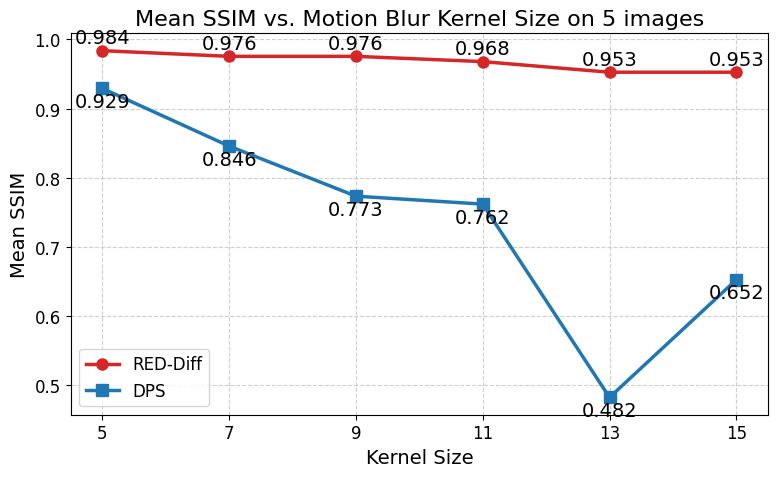
\includegraphics[width=0.5\textwidth]{media/mean_ssim_over_kernels.png}
        \caption{SSIM values for DPS and RED-Diff across different kernel sizes.}
        \label{fig:ssim_results}
    \end{figure}
\end{frame}

\begin{frame}{Performance Analysis}
    \begin{itemize}
        \item \textbf{Trend Analysis}:
              \begin{itemize}
                  \item Both methods show performance degradation with larger kernels, even though the RED-Diff method generally outperforms DPS.
                  \item PSNR and SSIM correlate with blur severity
              \end{itemize}
    \end{itemize}
\end{frame}

\begin{frame}{Visual Results Summary}
    \begin{itemize}
        \item \textbf{Qualitative Assessment}:
              \begin{itemize}
                  \item Side-by-side comparisons: Original → Blurred → Reconstructed
                  \item Visual quality correlation with quantitative metrics
                  \item Edge preservation and artifact analysis
              \end{itemize}
        \item \textbf{Key Findings}:
              \begin{itemize}
                  \item RED-Diff better preserves fine details
                  \item RED-Diff shows less artifacts compared to DPS
                  \item RED-Diff keeps consistent performances across different kernel sizes
                  \item DPS is more sensitive to kernel size variations, as shown in the PSNR and SSIM results
              \end{itemize}
    \end{itemize}
\end{frame}